\subsection{TET Histograms and Distance}
	Comparing the TET can be done in different ways. One of the method used to find similarity between the TETs is to transform the TET into a histogram is representing the by using the vector representation from \autoref{Eq:TETvector} we can calculate each substructures percentile distribution. this would give a representation as \autoref{fig:Tethistogram}
	
	\begin{figure}[H]
		\centering
		\begin{adjustbox}{width=0.5\textwidth}
			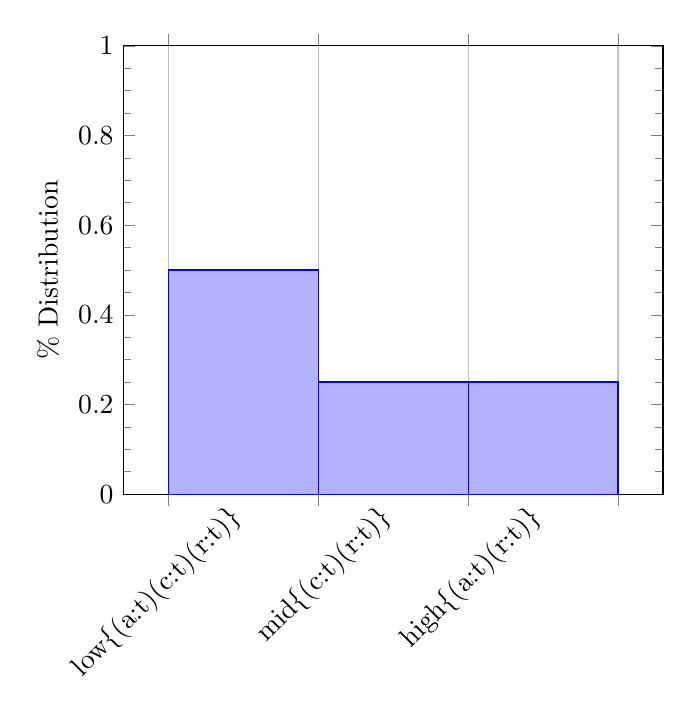
\begin{tikzpicture}
	\begin{axis}[
	ybar interval, 
	ymax=1,ymin=0, 
	minor y tick num = 3,
	ylabel = {\% Distribution},
	symbolic x coords={low\{(a:t)(c:t)(r:t)\}, mid\{(c:t)(r:t)\}, high\{(a:t)(r:t)\}, high\{(y:t)(r:t)\}},
	x tick label style={font=\normalsize, rotate=45, anchor=east},
	]
	\addplot coordinates {(low\{(a:t)(c:t)(r:t)\}, 0.5) (mid\{(c:t)(r:t)\}, 0.25) (high\{(a:t)(r:t)\}, 0.25) (high\{(y:t)(r:t)\}, 0.10)};
	\end{axis}
\end{tikzpicture}

%\begin{tikzpicture}

%\definecolor{bblue}{HTML}{4F81BD}

%\begin{axis}[
%major x tick style = transparent,
%ymin=0,
%bar width=1cm,
%minor y tick num = 3,
%ymajorgrids = true,
%ylabel = {\% distribution},
%symbolic x coords={low\{(a:t)(c:t)(r:t)\}, mid\{(c:t)(r:t)\}, high\{(a:t)(r:t)\}},
%xtick = data,
%x tick label style={font=\normalsize, rotate=45, anchor=east},
%]
%\addplot[ybar , style={bblue,fill=bblue,mark=none}]
%coordinates {(low\{(a:t)(c:t)(r:t)\}, 0.5) (mid\{(c:t)(r:t)\}, 0.25) (high\{(a:t)(r:t)\}, 0.25)};

%\end{axis}
%\end{tikzpicture}
		\end{adjustbox}
		\caption{caption}
		\label{fig:Tethistogram}
	\end{figure}
	
	By using this representation as a vector we can compare two histograms with simple distance measures as forekamle manhatten or euclidean distance.
	
	when comparing two histograms, one might have some elements that the other does not have. For any missing element in a histogram we add the value $0$, and we are thereby able to calculate distance for the missing element. A simple example done with manhattan distance can be seen in \autoref{Eq:manhattencomparason}.
	
	\begin{equation}\label{Eq:manhattencomparason}
	D(\begin{bmatrix}
	x_{1.1} \\
	x_{1.2} \\
	\end{bmatrix},
	\begin{bmatrix}
	x_{2.1} \\
	x_{2.2} \\
	x_{2.3}
	\end{bmatrix})= |x_{1.1} - x_{2.1}| + |x_{1.2} - x_{2.2}| + |0 - x_{2.3}|
	\end{equation}
	
	This is easily implemented if the vectors are programmed as dictionaries by going through, the union of keywords in the two dictionaries and returning 0 it a key is not found.
